% context: 9th-grade physics classwork, Unit 2 kinematics; review on 19 November
%        2026, the day before the unit test 2-11Test_Kinematics. Practice twin of the
%        test's two parabola problems (Q8 and Q9), with new numbers and contexts.
%        Open notes: no formulas printed
% topic: reading labelled points on a height-time parabola (top, rising and falling,
%        chord slope as average velocity, velocities at equal heights); deriving
%        y = v0 t - 5t^2, computing a table, plotting the parabola and its velocity
%        line
% structure: two pages; p1 the labelled parabola (easier); p2 table and both graphs
%        to plot (harder)
% data: chosen values. g = 10 m/s^2 so the points land on grid lines, as in 2-7CW.
%        Q1 rocket 40 m/s (top 80 m at 4 s); Q2 ball 10 m/s (top 5.0 m at 1.0 s, on
%        a table column). The test uses 30 m/s and 8 m/s
\documentclass[12pt, twoside]{article}
%\documentclass[12pt, twoside]{article}
\usepackage[letterpaper, margin=1in, headsep=0.2in]{geometry}
\setlength{\headheight}{0.6in}
%\usepackage[english]{babel}
\usepackage[utf8]{inputenc}
\usepackage{microtype}
\usepackage{amsmath}
\usepackage{amssymb}
%\usepackage{amsfonts}
\usepackage[nomessages]{fp} %\FPeval{\var-name}{2*sin(pi/6)}
\usepackage{siunitx} %units in math. eg 20\milli\meter
\usepackage{yhmath} % for arcs, overparenth command
\usepackage{tikz} %graphics
\usetikzlibrary{quotes, angles, arrows, arrows.meta}
\usepackage{graphicx} %consider setting \graphicspath{{images/}}
\usepackage{parskip} %no paragraph indent
\usepackage{enumitem}
\usepackage{multicol}
\usepackage{venndiagram}

\usepackage{fancyhdr}
\pagestyle{fancy}
\fancyhf{}
\renewcommand{\headrulewidth}{0pt} % disable the underline of the header
\raggedbottom
\hfuzz=2mm %suppresses overfull box warnings

\usepackage{hyperref}
\usepackage{float}

\title{Physics}
\author{Chris Huson}
\date{November 2026}

\fancyhead[LE]{\thepage}
\fancyhead[RO]{\thepage \\ Nickname: \hspace{2.25cm} \,\\ \,}
\fancyhead[LO]{La Scuola d'Italia / Huson / Physics \\* 19 November 2026}

\begin{document}

\subsubsection*{2.10 Classwork: Graphical Analysis}

Use your notes. Take \emph{up} as positive, and round $g$ to 10 m/s$^2$. Show your
work, with units.

\vspace{0.1cm}

\begin{enumerate}[itemsep=0.6cm]

\item A toy rocket is fired straight up from its launcher at 40 m/s. Ignore air
  resistance. The graph shows its height above the launcher. The labelled points
  sit on grid lines.

  \begin{center}
  \begin{tikzpicture}[x=1.5cm, y=0.064cm]
    \draw[gray!25, thin, xstep=0.2, ystep=2] (0,0) grid (8.6,90);
    \draw[gray!60, xstep=1, ystep=10] (0,0) grid (8.6,90);
    \draw[->, thick] (0,0) -- (8.9,0) node[right]{\small $t$ (s)};
    \draw[->, thick] (0,0) -- (0,94) node[above]{\small $y$ (m)};
    \foreach \t in {0,...,8} \node[below] at (\t,0) {\scriptsize \t};
    \foreach \y in {10,20,...,90} \node[left] at (0,\y) {\scriptsize \y};
    \draw[very thick, domain=0:8, samples=80] plot (\x, {40*\x - 5*\x*\x});
    \foreach \t/\y/\n/\p in {0/0/A/above left, 1/35/B/above left, 4/80/C/above,
        7/35/D/above right, 8/0/E/above right}
      { \fill (\t,\y) circle (3pt); \node[\p] at (\t,\y) {\textbf{\n}}; }
  \end{tikzpicture}
  \end{center}

  \begin{enumerate}[itemsep=0.4cm]
    \item Read the time and height of each labelled point.

      {\renewcommand{\arraystretch}{1.5}%
      \begin{tabular}{| l | p{1.3cm} | p{1.3cm} | p{1.3cm} | p{1.3cm} | p{1.3cm} |}
        \hline
        Point & \centering A & \centering B & \centering C & \centering D &
          \centering\arraybackslash E \\ \hline
        $t$ (s) & & & & & \\ \hline
        $y$ (m) & & & & & \\ \hline
      \end{tabular}}
    \item Which point is the top? What are the rocket's velocity and acceleration
      there?
      \vspace{0.6cm}
    \item Between which points is the rocket going up? Coming down? How does the
      graph show it?
      \vspace{0.6cm}
    \item Draw the chord from A to C. Find its slope. What does it tell you?
      \vspace{0.9cm}
    \item Find the rocket's velocity at B, at D and at E. Compare B and D.
      \vspace{0.9cm}
    \item Draw the chord from B to D. What is its slope? What does that mean?
  \end{enumerate}

\newpage

\item A ball is kicked straight up at 10 m/s. Take $y = 0$ where it is kicked.
  \begin{enumerate}[itemsep=0.4cm]
    \item Use your notes to show that the ball's height is $y = 10t - 5t^2$, and its
      velocity is $v = 10 - 10t$.
      \vspace{1.2cm}
    \item Fill in the table. Square the time first.

      {\renewcommand{\arraystretch}{1.5}%
      \setlength{\tabcolsep}{4pt}%
      \begin{tabular}{| l | p{0.85cm} | p{0.85cm} | p{0.85cm} | p{0.85cm} |
          p{0.85cm} | p{0.85cm} | p{0.85cm} | p{0.85cm} | p{0.85cm} | p{0.85cm} |
          p{0.85cm} |}
        \hline
        $t$ (s) & \centering 0 & \centering 0.2 & \centering 0.4 & \centering 0.6 &
          \centering 0.8 & \centering 1.0 & \centering 1.2 & \centering 1.4 &
          \centering 1.6 & \centering 1.8 & \centering\arraybackslash 2.0 \\ \hline
        $y$ (m) & & & & & & & & & & & \\ \hline
        $v$ (m/s) & & & & & & & & & & & \\ \hline
      \end{tabular}}
    \item Plot $y$ against $t$ on the position grid, and join the points with a
      smooth curve. Plot $v$ against $t$ on the velocity grid, and join the points
      with a ruler.

      \begin{tikzpicture}[x=2.65cm, y=1.2cm]
        \draw[gray!25, thin, xstep=0.1, ystep=0.2] (0,0) grid (2.0,5.6);
        \draw[gray!60, xstep=0.2, ystep=1] (0,0) grid (2.0,5.6);
        \draw[->, thick] (0,0) -- (2.1,0) node[below right]{\small $t$ (s)};
        \draw[->, thick] (0,0) -- (0,5.8) node[above]{\small $y$ (m)};
        \foreach \t in {0,0.4,0.8,1.2,1.6,2.0} \node[below] at (\t,0) {\scriptsize \t};
        \foreach \y in {1,...,5} \node[left] at (0,\y) {\scriptsize \y};
        \node[above] at (1.0,5.8) {\small Position};
        % Solution curve — uncomment to see the answer
        %\draw[very thick, domain=0:2, samples=60] plot (\x, {10*\x - 5*\x*\x});
        %\foreach \t in {0,0.2,...,2.0} \fill (\t, {10*\t - 5*\t*\t}) circle (1.5pt);
      \end{tikzpicture}
      \hfill
      \begin{tikzpicture}[x=2.65cm, y=0.335cm]
        \draw[gray!25, thin, xstep=0.1, ystep=1] (0,-10) grid (2.0,10);
        \draw[gray!60, xstep=0.2, ystep=2] (0,-10) grid (2.0,10);
        \draw[->, thick] (0,0) -- (2.1,0) node[above right]{\small $t$ (s)};
        \draw[->, thick] (0,-10) -- (0,11) node[above]{\small $v$ (m/s)};
        \foreach \t in {0.4,0.8,1.2,1.6,2.0}
          \node[below, fill=white, inner sep=1pt] at (\t,-0.3) {\scriptsize \t};
        \foreach \v in {-10,-8,-6,-4,-2,2,4,6,8,10} \node[left] at (0,\v) {\scriptsize \v};
        \node[above] at (1.0,11) {\small Velocity};
        % Solution line — uncomment to see the answer
        %\draw[very thick] (0,10) -- (2,-10);
        %\foreach \t in {0,0.2,...,2.0} \fill (\t, {10 - 10*\t}) circle (1.5pt);
      \end{tikzpicture}
    \item When is the ball highest, and how high does it go? What is its velocity
      at that moment?
      \vspace{0.8cm}
    \item Find the slope of the velocity graph, with units. What quantity is it?
  \end{enumerate}

\end{enumerate}
\end{document}
